\chapter{Dataset}
In total two datasets were created, one for detection of dental caries and the other for semantic segmentation of dental restorations. Majority of work was done on the former.
\section{Dental caries}
The dataset was created by MDDr. Tichy and his team. The work on the dataset began in Septmeber 2021 together with work on this thesis and we were thus able to discuss the format of the data. We decided to annotate every dental caries lession by minimal bounding box. Annotation process was conducted in Computer Vision Annotation Tool (CVAT), which was running on the server of Faculty of biomedical informatics, the web adress is gdiag.fbmi.cvut.cz.
\newline
Due to constant work on the dataset we decided to given data as long as there was no major update. This ensured, that we could compare performance of our models between each other, until a major update was released. In total, sig major releases were done, we will call those stages of the dataset.

\subsubsection{First stage}
In the first stage MDDr. Tichy instructed a group of students of general dentistry, how to approach the annotation to get as homogenous dataset as possible. The main goals were as follow:
\begin{itemize}
    \item Draw rectangular-shaped box around carious lession. The whole lession lies inside the box and the box is as tight as possible around the lession.
    \item When the lession is in proximal surface and booth teeth are infected, draw a separate box for each of them.
    \item When a tooth a major part of tooth is missing due to advanced decay of the teeth, do not try to estimate the height of the missing teeth, but draw a box
\end{itemize}
Dental X-ray images were uploaded into CVAT and seprated into multiple projects, where each project contained between 400-800 images. This was done due to technical limitation regarding exporting and uploading of X-ray images from a dental database. Each project was further split into jobs, each of them consisting of 100 images and assigned to a particular student. When the first stage was done we had 1695 X-ray images at our disposal with 2416 dental caries annotated. CVAT does not allow to export and merge multiple tasks, so that each task was exported separately in COCO format. All tasks were uploaded to CMP server and merged together. We checkcked the task for duplicit images and removed them, furthermore we removed any images, that were no yet review. This resulted in 1626 images with 2399 decay annotations, from those only 946 images contained at least one cavity.


\subsubsection{Second stage}
After inspection of the dataset created in the first stage we observed in-homogenity across annotations. Some of the guidilines were violated, especially annotation of caries in proximal surfaces was error-prone. In addition, multiple overlooked lession were observed. This led us to reconsideration of out approach to labeling and MDDr Tichy himself did all the annotation work from this moment forther on. After the second stage, the dataset was extended to 2599 non-duplicit images contatining 4328 annotation of tooth decay. In this stage no corrections of previous errors were done.

\subsubsection{Third stage}
All images annotated in the first stage were reviewed by MDDr. Tichy. Unspecified amount of annotations was removed as well as added. In the end the dataset consited of 2599 images with 4575 annotations of dental caries.

\subsubsection{Fourth stage}
Another 1400 images were uploaded onto CVAT server. After training the model on the dataset created in stage three, the model achieved performance of $AP@.5=0.61$. We downloaded all newly uploaded images and used the model to make predictions for those images. Confidence threshold achieving best results on the validation dataset was used to filter out low-confidence predictions. We used Voxel Fiftyone tool to upload all 1400 images and their respective predictions to CVAT, where those images were splitted into two seprate tasks.
MDDr Tichy review all predictions. Adjustments of bounding boxes as well as their removal and addition of were conducted. According to personal statistics of MDDr. Tichy, there were roughly 200 predictions per 100 images. Around 20 annotation had to be added and removed in order to get the same quality annotations as in stage three. Upside of this approach was speed, when annotation could be done in approximately half the time required to do the annotation without model predictions. In total 3500 images were available after this stage. After removal of corrupted images we got 3489 images with 6087 annotations of carious lessions.

\subsubsection{Fifth stage}
In this stage annotation of all 1400 images uploaded in stage four was finished, resulting in 3989 X-rays with 7257 annotations.

\begin{table}
    \centering
    \begin{tabular}{l|r|r}
                                       & Width [px] & Height [px] \\\hline
        Image size                     & 1068       & 795-847     \\ \hline
        Minimal box size               & 8          & 9           \\ \hline
        Maximal box size               & 384        & 315         \\ \hline
        Mean of box size               & 47.55      & 53.15       \\ \hline
        Standard deviation of box size & 37.99      & 35.33       \\ \hline
    \end{tabular}
    \caption{\label{tab:dataset_statistics}Staticstcs of dental caries annotations in the dataset}
\end{table}

\subsubsection{Sixth stage}
We evaluated performance of out model on test, validation and training part of the dataset. Despite the model used for prediction achieved $AP@.5 = 0.72$, there were 1598 images with at least one false positive or false negative detection. We decided, that doing second round of dataset review would be more benefitial, than further expansion of dataset size. We decided to focus only on errorneous images and uploaded 1598 images with at least single error to CVAT annotation tool for a review.

\

\section{Dental restorations}
\begin{figure}
    \centering
    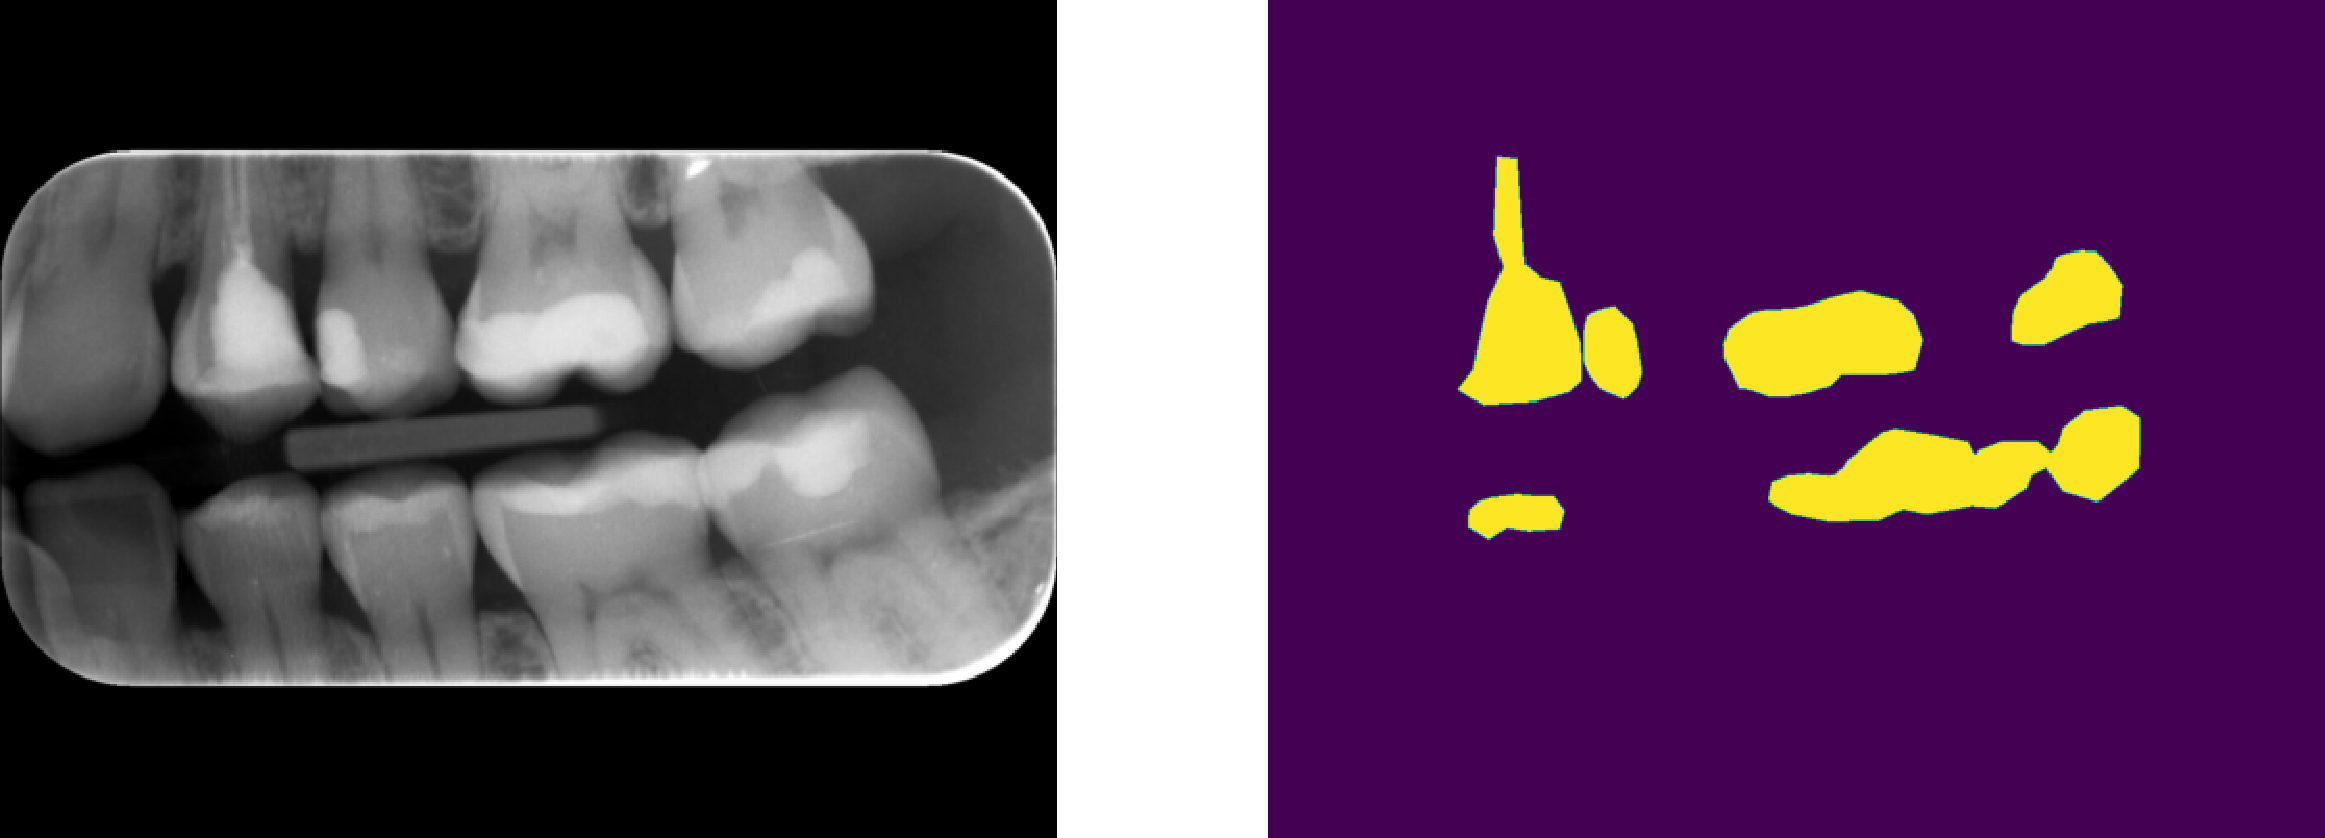
\includegraphics[width=\linewidth]{images/segmentation_ds_sample.pdf}
    \caption{Bitweing X-ray image on the left, pixel mask of the X-ray on the right (dental restorations have yellow color)}
    \label{fig:segmentation_sample}
\end{figure}
This dataset consists of subset of images used in the dental caries dataset. It was annotated in the CVAT tool, by drawing polygons around each dental restoration. The work was done by the same group of dentistry students as stage one of the caries dataset and reviewed by single fith-year dentistry student. Reviewing the whole dataset by single person should ensure consistency among images. Total of 521 images were used to create this dataset, 387 of them contained at least single annotated restoration and 134 contain none.
The dataset was exported from CVAT in COCO format and saved on CMP server. When working with the data we used pixel mask insted of polygons, to denote position of dental restorations. Sample of dataset with pixel mask can be seen in figure \ref{fig:segmentation_sample}.

In figure \ref{fig:segmentation_restoration_size} we can see, how many percent of X-ray image consists of restorations. This gives us an idea, how common restorations in our data are. In figure \ref{fig:segmentation_patch_size} we see, how size of individual restorations is distributed. Inspectiong this figure we observe, that majority of restorations is smaller, than $2\%$ of the image.

\begin{figure}
    \centering
    \begin{floatrow}[2]
        \ffigbox[\FBwidth]{\caption{Histogram of restoration area in image, images without restorations omited}\label{fig:segmentation_restoration_size}}%
        % {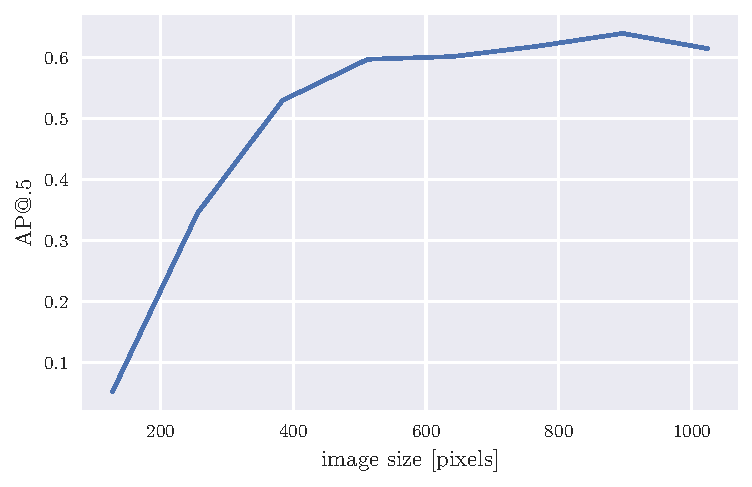
\includegraphics{images/img_size_dependency.pdf}}\qquad
        {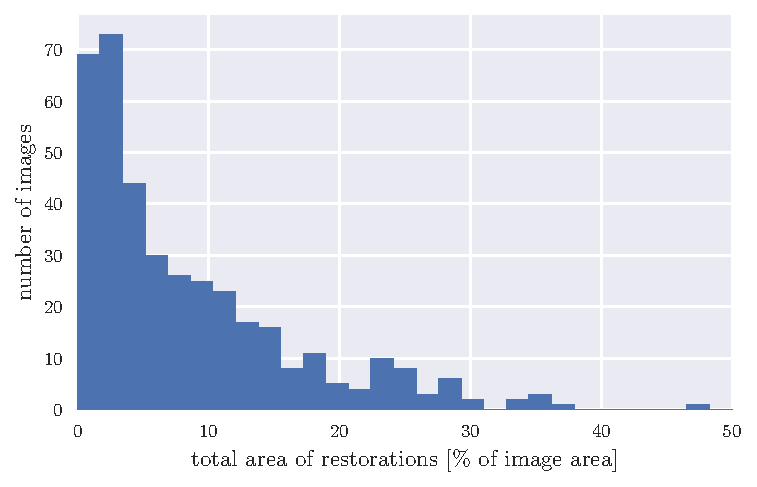
\includegraphics[width=\linewidth]{images/histogram_of_restoration_size.pdf}}\;
        % \ffigbox[\FBwidth]{\caption{Piero di Cosimo: \emph{Portrait of Simonetta Vespucci} (ca 1480)}}%
        % {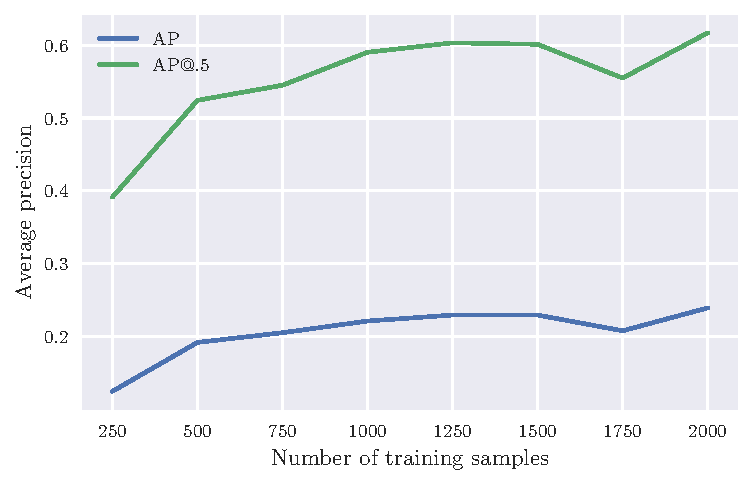
\includegraphics{images/training_set_dependency.pdf}}
        \ffigbox[\FBwidth]{\caption{Histogram of areas of restorations, 10 largest omited}\label{fig:segmentation_patch_size}}
        {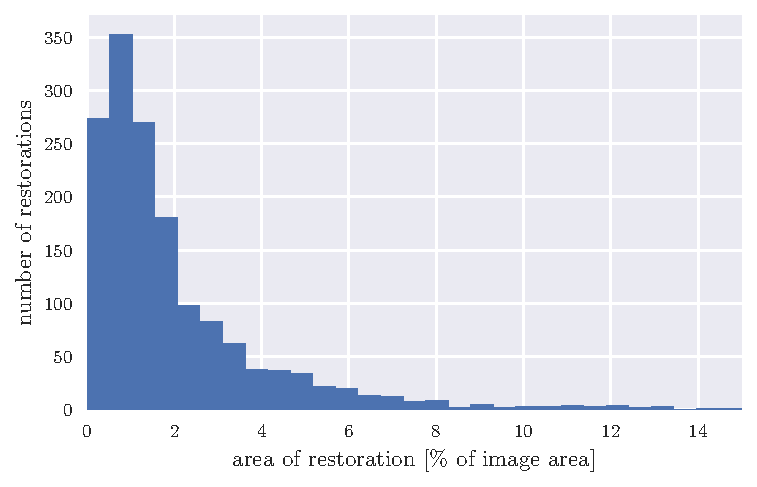
\includegraphics[width=\linewidth]{images/histogram_of_patch_size.pdf}}
    \end{floatrow}
\end{figure}